% Created by tikzDevice version 0.11 on 2018-05-19 10:30:07
% !TEX encoding = UTF-8 Unicode
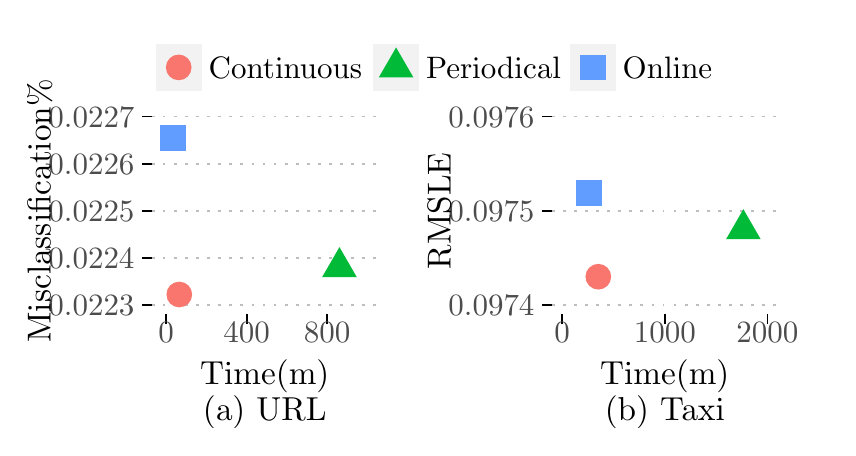
\begin{tikzpicture}[x=1pt,y=1pt]
\definecolor{fillColor}{RGB}{255,255,255}
\path[use as bounding box,fill=fillColor,fill opacity=0.00] (0,0) rectangle (289.08,144.54);
\begin{scope}
\path[clip] (  0.00,  0.00) rectangle (289.08,144.54);
\definecolor{fillColor}{RGB}{255,255,255}

\path[fill=fillColor] ( 35.88,115.81) rectangle (253.20,144.54);
\end{scope}
\begin{scope}
\path[clip] (  0.00,  0.00) rectangle (289.08,144.54);
\definecolor{drawColor}{RGB}{0,0,0}

\node[text=drawColor,anchor=base west,inner sep=0pt, outer sep=0pt, scale=  0.00] at ( 41.57,130.18) {Deployment};
\end{scope}
\begin{scope}
\path[clip] (  0.00,  0.00) rectangle (289.08,144.54);
\definecolor{drawColor}{RGB}{255,255,255}
\definecolor{fillColor}{gray}{0.95}

\path[draw=drawColor,line width= 0.6pt,line join=round,line cap=round,fill=fillColor] ( 45.90,121.50) rectangle ( 63.25,138.85);
\end{scope}
\begin{scope}
\path[clip] (  0.00,  0.00) rectangle (289.08,144.54);
\definecolor{fillColor}{RGB}{248,118,109}

\path[fill=fillColor] ( 54.58,130.18) circle (  4.64);
\end{scope}
\begin{scope}
\path[clip] (  0.00,  0.00) rectangle (289.08,144.54);
\definecolor{drawColor}{RGB}{255,255,255}
\definecolor{fillColor}{gray}{0.95}

\path[draw=drawColor,line width= 0.6pt,line join=round,line cap=round,fill=fillColor] (124.46,121.50) rectangle (141.80,138.85);
\end{scope}
\begin{scope}
\path[clip] (  0.00,  0.00) rectangle (289.08,144.54);
\definecolor{fillColor}{RGB}{0,186,56}

\path[fill=fillColor] (133.13,137.39) --
	(139.38,126.57) --
	(126.88,126.57) --
	cycle;
\end{scope}
\begin{scope}
\path[clip] (  0.00,  0.00) rectangle (289.08,144.54);
\definecolor{drawColor}{RGB}{255,255,255}
\definecolor{fillColor}{gray}{0.95}

\path[draw=drawColor,line width= 0.6pt,line join=round,line cap=round,fill=fillColor] (195.50,121.50) rectangle (212.85,138.85);
\end{scope}
\begin{scope}
\path[clip] (  0.00,  0.00) rectangle (289.08,144.54);
\definecolor{fillColor}{RGB}{97,156,255}

\path[fill=fillColor] (199.54,125.54) --
	(208.82,125.54) --
	(208.82,134.82) --
	(199.54,134.82) --
	cycle;
\end{scope}
\begin{scope}
\path[clip] (  0.00,  0.00) rectangle (289.08,144.54);
\definecolor{drawColor}{RGB}{0,0,0}

\node[text=drawColor,anchor=base west,inner sep=0pt, outer sep=0pt, scale=  1.12] at ( 65.42,126.32) {Continuous};
\end{scope}
\begin{scope}
\path[clip] (  0.00,  0.00) rectangle (289.08,144.54);
\definecolor{drawColor}{RGB}{0,0,0}

\node[text=drawColor,anchor=base west,inner sep=0pt, outer sep=0pt, scale=  1.12] at (143.97,126.32) {Periodical};
\end{scope}
\begin{scope}
\path[clip] (  0.00,  0.00) rectangle (289.08,144.54);
\definecolor{drawColor}{RGB}{0,0,0}

\node[text=drawColor,anchor=base west,inner sep=0pt, outer sep=0pt, scale=  1.12] at (215.02,126.32) {Online};
\end{scope}
\begin{scope}
\path[clip] (  0.00,  0.00) rectangle (144.54,115.81);
\definecolor{drawColor}{RGB}{255,255,255}
\definecolor{fillColor}{RGB}{255,255,255}

\path[draw=drawColor,line width= 0.6pt,line join=round,line cap=round,fill=fillColor] ( -0.00,  0.00) rectangle (144.54,115.81);
\end{scope}
\begin{scope}
\path[clip] ( 44.90, 40.93) rectangle (126.47,115.81);
\definecolor{fillColor}{RGB}{255,255,255}

\path[fill=fillColor] ( 44.90, 40.93) rectangle (126.47,115.81);
\definecolor{drawColor}{RGB}{255,255,255}

\path[draw=drawColor,line width= 0.3pt,line join=round] ( 44.90, 52.84) --
	(126.47, 52.84);

\path[draw=drawColor,line width= 0.3pt,line join=round] ( 44.90, 69.86) --
	(126.47, 69.86);

\path[draw=drawColor,line width= 0.3pt,line join=round] ( 44.90, 86.88) --
	(126.47, 86.88);

\path[draw=drawColor,line width= 0.3pt,line join=round] ( 44.90,103.90) --
	(126.47,103.90);

\path[draw=drawColor,line width= 0.3pt,line join=round] ( 64.60, 40.93) --
	( 64.60,115.81);

\path[draw=drawColor,line width= 0.3pt,line join=round] ( 93.68, 40.93) --
	( 93.68,115.81);

\path[draw=drawColor,line width= 0.3pt,line join=round] (122.76, 40.93) --
	(122.76,115.81);
\definecolor{drawColor}{RGB}{190,190,190}

\path[draw=drawColor,line width= 0.6pt,dash pattern=on 1pt off 3pt ,line join=round] ( 44.90, 44.34) --
	(126.47, 44.34);

\path[draw=drawColor,line width= 0.6pt,dash pattern=on 1pt off 3pt ,line join=round] ( 44.90, 61.35) --
	(126.47, 61.35);

\path[draw=drawColor,line width= 0.6pt,dash pattern=on 1pt off 3pt ,line join=round] ( 44.90, 78.37) --
	(126.47, 78.37);

\path[draw=drawColor,line width= 0.6pt,dash pattern=on 1pt off 3pt ,line join=round] ( 44.90, 95.39) --
	(126.47, 95.39);

\path[draw=drawColor,line width= 0.6pt,dash pattern=on 1pt off 3pt ,line join=round] ( 44.90,112.41) --
	(126.47,112.41);
\definecolor{drawColor}{RGB}{255,255,255}

\path[draw=drawColor,line width= 0.6pt,line join=round] ( 50.06, 40.93) --
	( 50.06,115.81);

\path[draw=drawColor,line width= 0.6pt,line join=round] ( 79.14, 40.93) --
	( 79.14,115.81);

\path[draw=drawColor,line width= 0.6pt,line join=round] (108.22, 40.93) --
	(108.22,115.81);
\definecolor{fillColor}{RGB}{97,156,255}

\path[fill=fillColor] ( 47.95,100.03) --
	( 57.23,100.03) --
	( 57.23,109.31) --
	( 47.95,109.31) --
	cycle;
\definecolor{fillColor}{RGB}{0,186,56}

\path[fill=fillColor] (112.66, 65.26) --
	(118.91, 54.43) --
	(106.41, 54.43) --
	cycle;
\definecolor{fillColor}{RGB}{248,118,109}

\path[fill=fillColor] ( 54.79, 48.12) circle (  4.64);
\end{scope}
\begin{scope}
\path[clip] (  0.00,  0.00) rectangle (289.08,144.54);
\definecolor{drawColor}{gray}{0.30}

\node[text=drawColor,anchor=base east,inner sep=0pt, outer sep=0pt, scale=  1.12] at ( 38.60, 40.48) {0.0223};

\node[text=drawColor,anchor=base east,inner sep=0pt, outer sep=0pt, scale=  1.12] at ( 38.60, 57.50) {0.0224};

\node[text=drawColor,anchor=base east,inner sep=0pt, outer sep=0pt, scale=  1.12] at ( 38.60, 74.52) {0.0225};

\node[text=drawColor,anchor=base east,inner sep=0pt, outer sep=0pt, scale=  1.12] at ( 38.60, 91.53) {0.0226};

\node[text=drawColor,anchor=base east,inner sep=0pt, outer sep=0pt, scale=  1.12] at ( 38.60,108.55) {0.0227};
\end{scope}
\begin{scope}
\path[clip] (  0.00,  0.00) rectangle (289.08,144.54);
\definecolor{drawColor}{RGB}{0,0,0}

\path[draw=drawColor,line width= 0.6pt,line join=round] ( 41.40, 44.34) --
	( 44.90, 44.34);

\path[draw=drawColor,line width= 0.6pt,line join=round] ( 41.40, 61.35) --
	( 44.90, 61.35);

\path[draw=drawColor,line width= 0.6pt,line join=round] ( 41.40, 78.37) --
	( 44.90, 78.37);

\path[draw=drawColor,line width= 0.6pt,line join=round] ( 41.40, 95.39) --
	( 44.90, 95.39);

\path[draw=drawColor,line width= 0.6pt,line join=round] ( 41.40,112.41) --
	( 44.90,112.41);
\end{scope}
\begin{scope}
\path[clip] (  0.00,  0.00) rectangle (289.08,144.54);
\definecolor{drawColor}{RGB}{0,0,0}

\path[draw=drawColor,line width= 0.6pt,line join=round] ( 50.06, 37.43) --
	( 50.06, 40.93);

\path[draw=drawColor,line width= 0.6pt,line join=round] ( 79.14, 37.43) --
	( 79.14, 40.93);

\path[draw=drawColor,line width= 0.6pt,line join=round] (108.22, 37.43) --
	(108.22, 40.93);
\end{scope}
\begin{scope}
\path[clip] (  0.00,  0.00) rectangle (289.08,144.54);
\definecolor{drawColor}{gray}{0.30}

\node[text=drawColor,anchor=base,inner sep=0pt, outer sep=0pt, scale=  1.12] at ( 50.06, 30.72) {0};

\node[text=drawColor,anchor=base,inner sep=0pt, outer sep=0pt, scale=  1.12] at ( 79.14, 30.72) {400};

\node[text=drawColor,anchor=base,inner sep=0pt, outer sep=0pt, scale=  1.12] at (108.22, 30.72) {800};
\end{scope}
\begin{scope}
\path[clip] (  0.00,  0.00) rectangle (289.08,144.54);
\definecolor{drawColor}{RGB}{0,0,0}

\node[text=drawColor,anchor=base,inner sep=0pt, outer sep=0pt, scale=  1.20] at ( 85.68, 15.45) {Time(m)};

\node[text=drawColor,anchor=base,inner sep=0pt, outer sep=0pt, scale=  1.20] at ( 85.68,  2.49) {(a) URL};
\end{scope}
\begin{scope}
\path[clip] (  0.00,  0.00) rectangle (289.08,144.54);
\definecolor{drawColor}{RGB}{0,0,0}

\node[text=drawColor,rotate= 90.00,anchor=base,inner sep=0pt, outer sep=0pt, scale=  1.20] at (  8.26, 78.37) {Misclassification\%};
\end{scope}
\begin{scope}
\path[clip] (144.54,  0.00) rectangle (289.08,115.81);
\definecolor{drawColor}{RGB}{255,255,255}
\definecolor{fillColor}{RGB}{255,255,255}

\path[draw=drawColor,line width= 0.6pt,line join=round,line cap=round,fill=fillColor] (144.54,  0.00) rectangle (289.08,115.81);
\end{scope}
\begin{scope}
\path[clip] (189.44, 40.93) rectangle (271.01,115.81);
\definecolor{fillColor}{RGB}{255,255,255}

\path[fill=fillColor] (189.44, 40.93) rectangle (271.01,115.81);
\definecolor{drawColor}{RGB}{255,255,255}

\path[draw=drawColor,line width= 0.3pt,line join=round] (189.44, 61.35) --
	(271.01, 61.35);

\path[draw=drawColor,line width= 0.3pt,line join=round] (189.44, 95.39) --
	(271.01, 95.39);

\path[draw=drawColor,line width= 0.3pt,line join=round] (211.68, 40.93) --
	(211.68,115.81);

\path[draw=drawColor,line width= 0.3pt,line join=round] (248.76, 40.93) --
	(248.76,115.81);
\definecolor{drawColor}{RGB}{190,190,190}

\path[draw=drawColor,line width= 0.6pt,dash pattern=on 1pt off 3pt ,line join=round] (189.44, 44.34) --
	(271.01, 44.34);

\path[draw=drawColor,line width= 0.6pt,dash pattern=on 1pt off 3pt ,line join=round] (189.44, 78.37) --
	(271.01, 78.37);

\path[draw=drawColor,line width= 0.6pt,dash pattern=on 1pt off 3pt ,line join=round] (189.44,112.41) --
	(271.01,112.41);
\definecolor{drawColor}{RGB}{255,255,255}

\path[draw=drawColor,line width= 0.6pt,line join=round] (193.14, 40.93) --
	(193.14,115.81);

\path[draw=drawColor,line width= 0.6pt,line join=round] (230.22, 40.93) --
	(230.22,115.81);

\path[draw=drawColor,line width= 0.6pt,line join=round] (267.30, 40.93) --
	(267.30,115.81);
\definecolor{fillColor}{RGB}{97,156,255}

\path[fill=fillColor] (198.24, 80.16) --
	(207.52, 80.16) --
	(207.52, 89.44) --
	(198.24, 89.44) --
	cycle;
\definecolor{fillColor}{RGB}{0,186,56}

\path[fill=fillColor] (258.62, 78.95) --
	(264.86, 68.12) --
	(252.37, 68.12) --
	cycle;
\definecolor{fillColor}{RGB}{248,118,109}

\path[fill=fillColor] (206.20, 54.55) circle (  4.64);
\end{scope}
\begin{scope}
\path[clip] (  0.00,  0.00) rectangle (289.08,144.54);
\definecolor{drawColor}{gray}{0.30}

\node[text=drawColor,anchor=base east,inner sep=0pt, outer sep=0pt, scale=  1.12] at (183.14, 40.48) {0.0974};

\node[text=drawColor,anchor=base east,inner sep=0pt, outer sep=0pt, scale=  1.12] at (183.14, 74.52) {0.0975};

\node[text=drawColor,anchor=base east,inner sep=0pt, outer sep=0pt, scale=  1.12] at (183.14,108.55) {0.0976};
\end{scope}
\begin{scope}
\path[clip] (  0.00,  0.00) rectangle (289.08,144.54);
\definecolor{drawColor}{RGB}{0,0,0}

\path[draw=drawColor,line width= 0.6pt,line join=round] (185.94, 44.34) --
	(189.44, 44.34);

\path[draw=drawColor,line width= 0.6pt,line join=round] (185.94, 78.37) --
	(189.44, 78.37);

\path[draw=drawColor,line width= 0.6pt,line join=round] (185.94,112.41) --
	(189.44,112.41);
\end{scope}
\begin{scope}
\path[clip] (  0.00,  0.00) rectangle (289.08,144.54);
\definecolor{drawColor}{RGB}{0,0,0}

\path[draw=drawColor,line width= 0.6pt,line join=round] (193.14, 37.43) --
	(193.14, 40.93);

\path[draw=drawColor,line width= 0.6pt,line join=round] (230.22, 37.43) --
	(230.22, 40.93);

\path[draw=drawColor,line width= 0.6pt,line join=round] (267.30, 37.43) --
	(267.30, 40.93);
\end{scope}
\begin{scope}
\path[clip] (  0.00,  0.00) rectangle (289.08,144.54);
\definecolor{drawColor}{gray}{0.30}

\node[text=drawColor,anchor=base,inner sep=0pt, outer sep=0pt, scale=  1.12] at (193.14, 30.72) {0};

\node[text=drawColor,anchor=base,inner sep=0pt, outer sep=0pt, scale=  1.12] at (230.22, 30.72) {1000};

\node[text=drawColor,anchor=base,inner sep=0pt, outer sep=0pt, scale=  1.12] at (267.30, 30.72) {2000};
\end{scope}
\begin{scope}
\path[clip] (  0.00,  0.00) rectangle (289.08,144.54);
\definecolor{drawColor}{RGB}{0,0,0}

\node[text=drawColor,anchor=base,inner sep=0pt, outer sep=0pt, scale=  1.20] at (230.22, 15.45) {Time(m)};

\node[text=drawColor,anchor=base,inner sep=0pt, outer sep=0pt, scale=  1.20] at (230.22,  2.49) {(b) Taxi};
\end{scope}
\begin{scope}
\path[clip] (  0.00,  0.00) rectangle (289.08,144.54);
\definecolor{drawColor}{RGB}{0,0,0}

\node[text=drawColor,rotate= 90.00,anchor=base,inner sep=0pt, outer sep=0pt, scale=  1.20] at (152.80, 78.37) {RMSLE};
\end{scope}
\end{tikzpicture}
